\chapter{Noncyclic constructions and extended Haagerup}
\label{ch:related-categories}

The name Haagerup appears in several related mathematical problems.
Replacing the order-three group by another finite abelian group is one
operation. Extending the initial string of a principal graph is another.
Taking an orbifold or a Morita partner is a third. These operations
change different parts of the data, and their outputs need not belong
to one family of fusion rules.

This chapter develops two useful comparisons with the preceding
construction. Noncyclic Haagerup--Izumi coefficients illustrate how
signs, integer lifts, and exact polynomial certificates work together.
Extended Haagerup illustrates how a planar algebra can specify an
entire tensor category without printing all its associator matrices.
The small calculations will be explicit; the large finite certificates
will be identified as supplied inputs. Neither comparison supplies a
new conformal field theory.

\section{Keeping the fusion rules in view}
\index{Haagerup--Izumi construction!noncyclic groups}

For a finite abelian group $G$, put $n=|G|$. The generalized
Haagerup rules considered here have simples $A_g,R_g$, $g\in G$,
and the same formulas as \eqref{eq:HI-general-fusion}:
\[
 A_gA_h=A_{g+h},\qquad A_gR_h=R_{g+h},\qquad
 R_gA_h=R_{g-h},\qquad
 R_gR_h=A_{g-h}+\sum_{k\in G}R_k.
\]
There are $n$ invertible and $n$ noninvertible simples. The positive
dimension of every $R_g$ is
\[
 d_n=\frac{n+\sqrt{n^2+4}}2,
 \qquad \FPdim(\mathcal C)=n(1+d_n^2).
\]
The group law matters even when two groups have the same order.
For example, the invertibles for $\Z_8$ contain an element of order
eight, whereas those for $\Z_4\times\Z_2$ do not. Their fusion rings
are already different before choosing an associator.

For $|G|>1$, these also differ from \emph{near-group} rules, which have
only one noninvertible simple together with a group of invertibles.
The phrase ``related to Haagerup'' should therefore always be followed
by a statement of the simple objects and their fusion.

Even group order introduces an additional issue. The coefficient
presentation generally needs a family of matrices
$\mathsf A_g(p,q)$ and signs $\epsilon_h(g)$, rather than the
single untwisted matrix used in Chapter~\ref{ch:arithmetic}.
The index $g$ labels a \emph{sheet} of the coefficient data. It is
not an extra simple-object label beyond the displayed fusion ring.
Transport equations relate the sheets. The following construction
makes their signs concrete for certain rank-two group quotients.

\section{Why a determinant phase appears}
\index{reciprocal weights}

Take
\[
 \Lambda=\Z^2,\qquad \Gamma=2\Z\times2m\Z,
 \qquad G=\Lambda/\Gamma,\qquad n=4m,
\]
and choose either root $\delta$ of $\delta^2=n\delta+1$.
Write $\tau=\delta-1$ and
\[
 M=\begin{pmatrix}1&1\\0&1\end{pmatrix},\qquad
 J=\begin{pmatrix}0&1\\-1&0\end{pmatrix},\qquad
 \epsilon_h(g)=(-1)^{h^TMg}.
\]
Integer representatives are used until all signs have been evaluated.
The relation $M+M^T\equiv J\pmod2$ will make the phase cancellations
work.

An auxiliary weight is a nonzero function on integer lifts satisfying
\begin{align}
 W(0)&=-1,\notag\\
 W(a+2z)&=(-1)^{a^TMz}W(a)
       &&(2z\in\Gamma),\label{eq:noncyclic-monodromy}\\
 W(a)W(-a)&=\delta &&(a\notin\Gamma).
 \label{eq:noncyclic-reciprocity}
\end{align}
Thus $W$ is not quite a function on $G$: changing a lift can change
its sign. This prescribed change is called its monodromy here.
It is compatible with consecutive shifts because the extra cross
term in the exponent is even. At a lift of the zero class, the
weight is $-1$ and its reciprocal product is $1$, not $\delta$.

Define the parity correction
\[
 \sigma(a)=(-1)^{\lfloor a/2\rfloor^TM(a\bmod2)},\qquad
 D_g(p,q)=\sigma(g)\sigma(g+p)\sigma(g+q)\sigma(g+p+q),
\]
where division and remainder are coordinatewise. The useful identity is
\[
 \sigma(g+2h)/\sigma(g)=\epsilon_h(g).
\]
Now set
\begin{align}
 B(p,q)&=i^{\det(p,q)}\frac{W(p)W(q-p)}{W(q)}
 +\tau\mathbf1_{q\in\Gamma}(-1)^{(q/2)^TMp},
 \label{eq:noncyclic-B}\\
 \mathsf A_g(p,q)&=\tau^{-1}D_g(p,q)B(p,q).
 \label{eq:noncyclic-A}
\end{align}
The expression involving $q/2$ is used only when $q\in\Gamma$,
so its exponent is integral. The determinant couples the two
coordinates. Omitting it would change the coefficient identities.

\begin{example}[Descent from integer lifts]
Shift $p$ to $p+2z$ with $2z\in\Gamma$. The determinant and
weight factors in the first term of $B$ contribute the sign
\[
 (-1)^{\det(z,q)+p^TMz+(q-p)^TMz}
 =(-1)^{z^TMq}=\epsilon_z(q).
\]
The equality uses $M+M^T\equiv J\pmod2$. The exceptional term
has the same transformation. Meanwhile $D_g(p,q)$ acquires
exactly the same sign, so their product is unchanged. The $q$
shift works similarly, and changing the representative of $g$
leaves the whole expression unchanged. Thus $\mathsf A_g(p,q)$
is well defined on the finite group even though $W$ itself has
nontrivial monodromy.
\end{example}

Reciprocity gives the three axis values
\[
 B(p,0)=B(0,p)=B(p,p)=\tau\mathbf1_{p\in\Gamma}-1.
\]
For example, at $q=0$ and nonzero residue $p$, the weight quotient
is $-\delta$; adding $\tau$ changes it to $-1$. This explains
the exceptional correction in \eqref{eq:noncyclic-B}. In particular
\begin{equation}
 \mathsf A_g(p,0)=\mathbf1_{p=0}-\frac1{\delta-1},\qquad
 \sum_{p\in G}\mathsf A_g(p,0)=-\frac1\delta.
 \label{eq:noncyclic-axis}
\end{equation}
The last equality follows from $\delta^2=n\delta+1$.

The determinant ansatz solves the linear transport and rotation
equations for every admissible weight. It also gives the pointwise
identity
\begin{equation}
 \mathsf A_g(p,q)\mathsf A_g(q,p)
 =\frac{\delta}{(\delta-1)^2}
 \quad(p,q\ne0,\ p\ne q).
 \label{eq:noncyclic-pair}
\end{equation}
Here the determinant phases cancel and the remaining product is
$W(q-p)W(p-q)=\delta$. However, the summed quadratic and cubic
equations remain to be solved. Pointwise reciprocity is much less
information than a full recoupling identity.

\begin{example}[The Klein-four coefficient matrix]
For $m=1$, choose $t^2=-\delta$ and set $W(a)=t$ at the three
nonzero representatives. One solution has
\[
 (\delta-1)\mathsf A_0=
 \begin{pmatrix}
 \delta-2&-1&-1&-1\\
 -1&-1&-it&-it\\
 -1&-it&-1&-it\\
 -1&-it&-it&-1
 \end{pmatrix},\qquad \delta^2=4\delta+1,
\]
in the order $(0,0),(0,1),(1,0),(1,1)$. To see one phase,
take $p=(0,1)$ and $q=(1,0)$. The determinant is $-1$,
so its phase is $-i$; the monodromy rule and quotient of weights
give the remaining factor $t$.

At $\delta=2+\sqrt5$, choose $t=i\sqrt\delta$. Then
$-it=\sqrt\delta$ and the displayed matrix is real symmetric.
At the negative root $\delta=2-\sqrt5$, choose
$t=\sqrt{-\delta}>0$; its off-diagonal lower entries are
imaginary and do not satisfy the same Hermitian condition.
Polynomial transport to another embedding has preserved the
algebraic equations, not the original positive adjoint.

One quadratic normalization can be checked immediately:
\[
 \sum_{a\in G}\mathsf A_0(a,0)^2
 =\frac{(\delta-2)^2+3}{(\delta-1)^2}
 =1-\delta^{-1}.
\]
Indeed the numerator is $8$, the denominator is $2(\delta+1)$,
and $(5-\delta)(\delta+1)=4$. This one calculation illustrates
the dimension equation's role; the complete known Klein-four
solution requires all the remaining coefficient equations as well.
\end{example}

For odd $m$, the three nonzero elements of $G[2]$ have weights
whose squares equal $-\delta$. Multiplication of $W$ by a group
character changes no coefficient quotient. It can fix two of those
three signs, leaving one discrete sign. The other $4m-4$ elements
form $2m-2$ inverse pairs, giving that many independent nonzero
weights. At $m=3$, only four continuous parameters remain.

The same descent proof works for any finite-index
$\Gamma\subseteq2\Z^2$. This is a general theorem about the
\emph{linear ansatz}. It does not prove existence of solutions
to the nonlinear equations for every such quotient.

\section{Two different achievements at orders eight and twelve}

Before using cyclic order eight, one extension of the previous
chapter must be stated. The even-cyclic coefficient problem has
signed sheets. After removing their parity factors, a column of
the scalar kernel obeys
\[
 B(a+n,h)=(-1)^h B(a,h).
\]
Even columns are periodic and odd columns are antiperiodic.
Their finite Fourier bases therefore use frequencies
$k$ or $k+\tfrac12$, respectively: translating
$e^{2\pi i(k+1/2)a/n}$ by $n$ multiplies it by $-1$.
The same gamma function supplies the samples, but the frequency
bookkeeping has changed. The supplied even-cyclic analytic
manuscript proves the signed quadratic and cubic identities.
The order-eight calculation below imports its quadratic identities;
it does not reprove that analytic extension or claim that it belongs
to the all-odd Lean theorem described in the previous chapter.

\subsection{An exact special-function identification at order eight}

The group $\Z_4\times\Z_2$ has a published generalized Haagerup
construction. Its radical coefficients can be expressed using one
degree-eight scalar. A separate calculation in the supplied work
identifies its negative-embedding weights with products of the same
double-sine samples that occur in cyclic order eight. The category's
existence and this special-function identification are different
statements.

Put
\[
 D_8=4+\sqrt{17},\qquad t=D_8^{-1/2},\qquad
 F_k=\operatorname{Sin}_2\left(1+\frac{kD_8}{D_8+1};D_8,1\right).
\]
To fix the normalization without a naming ambiguity, use the gamma
of Chapter~\ref{ch:arithmetic} with periods
$\omega_1=D_8+1$, $\omega_2=1+D_8^{-1}$. Then
\[
 F_k=\gamma(\omega_2+k)^{-1}.
\]
Thus this double sine is the rescaled \emph{reciprocal} gamma;
its period shifts divide by the corresponding sine factors.
All samples used below lie in its positive real strip.
Set $y=F_2$ and $r=F_3/F_1$.
Four of the proved cyclic quadratic equations have the following
exact elimination consequences:
\begin{equation}
 y^2r^2=tr^2+2,\qquad
 2tr^4+(3-t^2)r^2-2t=0,
 \qquad t^4+8t^2-1=0.
 \label{eq:noncyclic-eight-eliminants}
\end{equation}
The finite elimination is a supplied rational ideal-membership
certificate. Once these two equations are available, the branch
identification can be done by hand.

Write $s=t^2=\sqrt{17}-4$. The second equation gives
\[
 r^{-2}-r^2=\frac{3-s}{2t}>0.
\]
Positivity of the gamma samples implies $0<r<1$. Using
$s^2+8s-1=0$ and squaring yields
\[
 r^2+r^{-2}=\frac{9+s}{2},\qquad
 r+r^{-1}=\frac{5+s}{2}.
\]
The positive square roots are forced at both steps. Thus
\begin{equation}
 r=\frac{1+\sqrt{17}-\sqrt{2+2\sqrt{17}}}{4}
 =:\lambda_8^2.
 \label{eq:noncyclic-lambda8}
\end{equation}
The quartic
$r^4-r^3-2r^2-r+1=0$, together with the second eliminant,
also gives $tr^3=1-2r$. The solution to
Exercise~\ref{ex:noncyclic-eight-branch} derives this identity
explicitly on the positive branch. Multiply the first eliminant by $r$:
$y^2r^3=tr^3+2r=1$. Since $y>0$,
\begin{equation}
 F_2=\lambda_8^{-3},\qquad F_3/F_1=\lambda_8^2.
 \label{eq:noncyclic-eight-gamma}
\end{equation}
This is an exact equality, not recognition from a decimal fit.
It also shows why an eliminant alone is insufficient: without
positivity one has not selected the correct reciprocal root or
the sign of $y$.

\subsection{An algebraic existence certificate at order twelve}

For $G=\Z_2\times\Z_6$, use
\[
 t=\sqrt{\sqrt{37}-6},\qquad
 \delta=-t^2=6-\sqrt{37},\qquad t^4+12t^2-1=0.
\]
The four unknown weights can be specified algebraically. A convenient
auxiliary variable $u$ is the unique root in $(3,4)$ of
\[
 u^3+t(t^2+13)u^2-(26+2t^2)u-t(48+4t^2)=0.
\]
For example, $2/7<t<3/10$ proves that the polynomial changes
sign between $3$ and $4$ and has positive derivative there.
Set $C=(u+\sqrt{u^2+4})/2$, so $u=C-C^{-1}$.
Clearing its inverse powers gives a monic sextic
\begin{align}
 P_t(C)={}&C^6+t(t^2+13)C^5-(29+2t^2)C^4
 -t(74+6t^2)C^3\notag\\
 &+(29+2t^2)C^2+t(t^2+13)C-1.
 \label{eq:noncyclic-twelve-sextic}
\end{align}

The supplied construction expresses the four normalized weights
$z_j$ as rational functions of $t,C$. The coefficient equations
can therefore be checked in the finite rational algebra
\begin{equation}
 E=\bigl(\Q[t]/(t^4+12t^2-1)\bigr)[C]/(P_t(C)).
 \label{eq:noncyclic-certificate-algebra}
\end{equation}
Its basis consists of the $24$ monomials $t^iC^j$, with
$0\leq i<4$ and $0\leq j<6$. We call this a finite algebra;
irreducibility is not needed for the verification method. An inverse
is accepted only with a polynomial B\'ezout identity proving its
denominator is a unit. After that, every asserted identity has
$24$ rational coefficients to check.

\begin{constructioninput}[The recorded order-twelve certificate]
\label{input:noncyclic-twelve}
The specified algebraic weights solve every signed transpose
coefficient equation for $\Z_2\times\Z_6$. Their $1,728$
indexed quadratics reduce to $16$ nonzero Laurent-polynomial
types, and their $248,832$ indexed cubics to $246$ types;
all remainders in \eqref{eq:noncyclic-certificate-algebra} vanish.
The recorded certificate includes a second extraction of the
indexed equations, nonvanishing denominators, and exact real
root isolation. These recorded finite checks are inputs to this
chapter; they have not been rerun while preparing the textbook.
\end{constructioninput}

There is a further exact step to unitarity. At positive dimension
$\delta_+=6+\sqrt{37}$, put $t=i\sqrt{\delta_+}$. The
certificate proves that all six roots $C$ of the sextic lie on the
unit circle. Hence ordinary conjugation acts by
\[
 t\longmapsto-t,\qquad C\longmapsto C^{-1}.
\]
It also proves $z_j(t,C)z_j(-t,C^{-1})=1$. Consequently every
normalized $z_j$ has modulus one. The nonzero representative
weights are $t$, $tz_j$, or signed $t/z_j$, and real sign
monodromy determines their other lifts. Thus every nonzero-residue
weight has squared modulus $\delta_+$.
Equation~\eqref{eq:noncyclic-pair} then upgrades to
\[
 \mathsf A_g(q,p)=\overline{\mathsf A_g(p,q)}.
\]
Indeed both the product and $|\mathsf A_g(p,q)|^2$ equal
$\delta_+/(\delta_+-1)^2$; divide by the nonzero first factor.
The axis entries are already real. This explains how a separate
conjugation certificate supplies information absent from the
polynomial equations alone.

With the corresponding reconstruction theorem, the recorded
result is a unitary category with $24$ simples and noninvertible
dimension $6+\sqrt{37}$. The fixed axis condition supplies the
$Q$-system $\one\oplus R_0$, giving subfactor index
$7+\sqrt{37}$. Six positive coefficient embeddings do not by
themselves mean six inequivalent categories: gauge changes and
group automorphisms must first be considered.

\begin{remark}[What remains open in the gamma formula]
Put $D_{12}=6+\sqrt{37}$ and use the corresponding double-sine
samples $F_k$ as above. The proposed negative-embedding identities are
\[
 (z_0,z_1,z_2,z_3)=
 \left(\frac{F_2F_5}{F_1},\frac{F_2}{F_4},
       \frac{F_2}{F_4^2},-\frac{F_5}{F_1}\right).
\]
They match the independently refined algebraic branch to high
precision, but their exact identification remains open in the
current source. The algebraic existence and unitarity certificate
does not depend on this conjecture. Conversely, a tiny residual
from these products does not prove their equality to the exact
weights. One relation follows immediately from the proposed
products, $z_0z_2+z_1^2z_3=0$; obtaining one such relation is
far short of the full coefficient system.
\end{remark}

\section{The same quadratic unit, two quotient groups}

There is a useful arithmetic reason to compare cyclic and noncyclic
examples at the same order. Let
\[
 D=2m+\sqrt{4m^2+1},\qquad
 \omega=\frac{1+\sqrt{4m^2+1}}2.
\]
Then $D=2\omega+2m-1$ and $\omega^2=\omega+m^2$.
The quadratic order $\Z[D]$ has index two in $\Z[\omega]$.
Imposing $D=1$ in $D^2-4mD-1=0$ gives
\[
 \Z[D]/(D-1)\Z[D]\cong\Z_{4m}.
\]
In the basis $(1,\omega)$, multiplication by $D-1$ instead has matrix
\[
 2\begin{pmatrix}m-1&m^2\\1&m\end{pmatrix}.
\]
Its entries have gcd $2$ and its determinant is $-4m$, so its
Smith invariant factors are $2$ and $2m$. Therefore
\begin{equation}
 \Z[\omega]/(D-1)\Z[\omega]
 \cong\Z_2\times\Z_{2m}
 \quad\hbox{as additive groups}.
 \label{eq:noncyclic-orders}
\end{equation}
At $m=1$ this compares $\Z_4$ with the Klein group; at $m=3$
it compares $\Z_{12}$ with $\Z_2\times\Z_6$. The dimension
parameter is the same while the group changes. This arithmetic
observation motivates the common special function. It does not
derive the weight formulas or solve the nonlinear equations.

\subsection{Why an auxiliary action's kernel need not shrink the group}

Reconstruction must recover exactly the $2|G|$ promised simples.
A subtlety arises when the signed group action on the first
auxiliary algebra has a kernel. One cannot simply identify the
corresponding group elements and continue to claim the original
fusion ring. The supplied algebraic reconstruction removes that
kernel by enlarging the auxiliary algebra.

Here is the mechanism. Start with the Leavitt algebra $L$ with
generators $s,t_g,s',t'_g$, whose relations say that the column
$(s,t_g)$ and row $(s',t'_g)$ are inverse rectangular matrices:
\[
 s's=1,\quad t'_gt_h=\delta_{g,h},\quad
 s't_g=t'_gs=0,\qquad ss'+\sum_gt_gt'_g=1.
\]
The primes are algebraic partners; they do not denote an adjoint.
The coefficient equations produce endomorphisms $\alpha_g,\rho$
obeying covariance and the splitting of $\rho^2$ on $L$.

Let $D=\C^G$ be functions on the finite group, with translations
$(\theta_gf)(x)=f(x-g)$. Form the unital algebraic free product
\[
 \mathcal B=L*_{\C}D_1*_{\C}D_2.
\]
This consists of finite linear combinations of alternating words
from the three factors, subject only to their own relations and
the common scalar unit. In particular every factor embeds. Extend
the action by
\[
 \widetilde\alpha_g(f_1)=(\theta_gf)_1,\qquad
 \widetilde\alpha_g(f_2)=(\theta_{-g}f)_2,
\]
and extend $\rho$ by
\[
 \widetilde\rho(f_1)=f_2,\qquad
 \widetilde\rho(f_2)=sf_1s'
       +\sum_gt_g(\theta_{-g}f)_2t'_g.
\]
The second expression preserves multiplication because distinct
Leavitt corners annihilate each other; it preserves the unit
because the corner projections sum to one. The free-product
universal property therefore gives an endomorphism. The extended
group action is faithful on $D_1$, regardless of its behavior on
$L$.

The full reconstruction proof checks covariance and
\[
 \widetilde\rho^2(b)=sbs'
       +\sum_gt_g\widetilde\alpha_g\widetilde\rho(b)t'_g
       \qquad(b\in\mathcal B).
\]
Checking this on each free factor suffices. On $D_1$ it is the
displayed definition; on $D_2$ the coefficient quadratics cancel
the mixed terms. A further intertwiner lemma shows that this
enlargement creates no unwanted intertwiners between the proposed
simple endomorphisms. Its useful idea is that an equation
$ux=xv$, with $u$ homogeneous of positive degree and left
invertible in $L$, cannot be satisfied by a nonzero component
of $x$ containing new free-product letters: it would produce a
finite-dimensional subspace invariant under multiplication by
$u$, contradicting the grading. These checks supply all the
group labels and their distinct simple objects.
The relevant grading is concrete:
$\deg s=2$, $\deg t_g=1$, $\deg s'=-2$, and
$\deg t'_g=-1$; every Leavitt relation is homogeneous.

This is an algebraic construction for the full signed transpose
system with $\eta_g=1$ and finite abelian $G$. It needs neither
an analytic completion nor a positive functional. A separate
positive Hermitian reconstruction is used for a unitary conclusion,
as in the order-twelve example. A repair of faithfulness is not
itself a proof of unitarity.

\section{Extended Haagerup changes the construction problem}
\index{Extended Haagerup}

Extended Haagerup comes from a different principal graph. Its
first branching occurs later: its planar algebra agrees with the
Temperley--Lieb diagrams through box degree seven, and an extra
generator first appears in degree eight. This property is called
\emph{seven-supertransitivity}. The corresponding Haagerup
example is three-supertransitive. The word ``extended'' refers
to the additional initial graph string.

Write $x$ for its subfactor index, reserving the fixed symbol
$d$ for the order-three Haagerup dimension elsewhere in this book:
\begin{equation}
 x=3+2\cos\frac{4\pi}{13}+2\cos\frac{6\pi}{13},\qquad
 x^3-8x^2+17x-5=0,
 \qquad x\approx4.37720.
 \label{eq:EH-index}
\end{equation}
The two original unitary even parts have ranks six and eight.
Their common global dimension is
\begin{equation}
 D_{\rm EH}=125x^2-450x+145,\qquad
 D_{\rm EH}^3-585D_{\rm EH}^2+8450D_{\rm EH}-21125=0.
 \label{eq:EH-global}
\end{equation}
The published Morita classification has four unitary categories,
of ranks $6,8,8,8$. The rank-six category is conventionally
$EH_1$ and the original rank-eight category $EH_2$.

\begin{proposition}[A dimension obstruction to identifying the families]
No category with the generalized Haagerup fusion rules above is
Morita equivalent to an extended Haagerup category.
\end{proposition}
\begin{proof}
For $n\geq1$ the generalized Haagerup global Frobenius--Perron
dimension is
\[
 n(1+d_n^2)=2n+n^2d_n.
\]
It has degree two over $\Q$, since $n^2+4$ is not a square.
The cubic for $D_{\rm EH}$ reduces modulo two to
$u^3+u^2+1$, which has no root in $\mathbb F_2$ and is
irreducible. Thus $D_{\rm EH}$ has degree three. Morita
equivalence preserves global Frobenius--Perron dimension, so
these numbers cannot be equal. The argument uses the positive
Frobenius--Perron dimension and remains valid for a nonunitary
categorification of the generalized Haagerup ring.
\end{proof}

The transferable idea is to construct finite exact tensor data and
then reconstruct a category. The specific group-indexed coefficient
system does not transfer to extended Haagerup.

\section{A planar algebra as a tensor presentation}
\index{planar algebra}
\index{Jones--Wenzl projection}

A shaded planar algebra assigns a vector space $P_{k,+}$ or
$P_{k,-}$ to a box with $2k$ boundary points. A diagram connecting
several boxes by nonintersecting strings defines a multilinear
operation on their labels. The signs specify the two checkerboard
shadings. Substitution of diagrams agrees with composition of the
corresponding operations. Vertical stacking gives multiplication,
horizontal placement gives tensor product, and closing strings
gives a trace. Reflection supplies the adjoint in a planar
$*$-algebra.

For a subfactor planar algebra the empty diagram is the scalar
identity in each zero-box space, and the trace pairing is positive.
In an ambient graph planar algebra there are several zero-box
coordinates, one for each vertex of the corresponding parity.
An identity asserted to equal a scalar there must hold with the
same scalar at every such vertex. Checking only one coordinate
would be insufficient.

Put $\beta=\sqrt x>2$ and define quantum integers by
\[
 [0]=0,\quad[1]=1,\quad [k+1]=\beta[k]-[k-1].
\]
A contractible string loop evaluates to $\beta$. The
Jones--Wenzl projection $f^{(k)}$ is the part of $k$ parallel
strands annihilated by every Temperley--Lieb turnback $e_i$,
which joins neighboring strands on the same side of the box.
Its trace is $[k+1]$. This turnback condition is different from
annihilation by every boundary cap: a Jones--Wenzl projection
has a nonzero partial trace.
The first nontrivial case can be derived without any machinery.
If $e$ joins two neighboring strands by a cup and cap, then
$e^2=\beta e$. Therefore
\[
 f^{(2)}=1-\beta^{-1}e,
 \qquad (f^{(2)})^2=f^{(2)},\qquad ef^{(2)}=0.
\]
\begin{figure}[htbp]
\centering
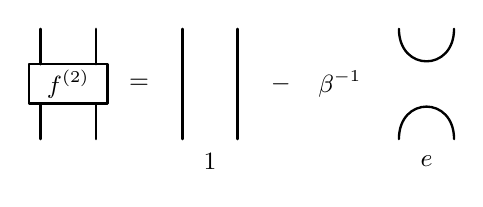
\begin{tikzpicture}[
  x=1cm,y=1cm,line width=0.85pt,
  line cap=round,line join=round,font=\small]
  % First row: the projector, identity, and cup--cap operator.
  % Each diagram has two inputs at y=0 and two outputs at y=1.4.
  \draw (0,0)--(0,0.45);
  \draw (0.7,0)--(0.7,0.45);
  \draw (0,0.95)--(0,1.4);
  \draw (0.7,0.95)--(0.7,1.4);
  \draw (-0.15,0.45) rectangle (0.85,0.95);
  \node at (0.35,0.7) {$f^{(2)}$};

  \node at (1.25,0.7) {$=$};
  \draw (1.8,0)--(1.8,1.4);
  \draw (2.5,0)--(2.5,1.4);
  \node at (2.15,-0.28) {$1$};

  \node at (3.05,0.7) {$-$};
  \node at (3.8,0.7) {$\beta^{-1}$};
  % Lower cap joins the two input endpoints; upper cup joins outputs.
  \draw (4.55,0)
    .. controls (4.55,0.55) and (5.25,0.55) .. (5.25,0);
  \draw (4.55,1.4)
    .. controls (4.55,0.85) and (5.25,0.85) .. (5.25,1.4);
  \node at (4.9,-0.28) {$e$};
\end{tikzpicture}

\smallskip

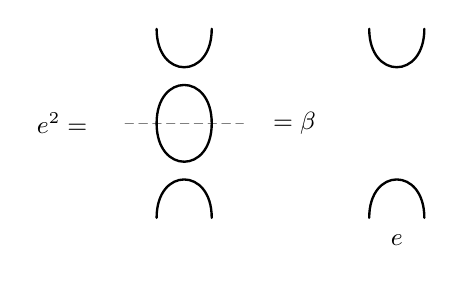
\begin{tikzpicture}[
  x=1cm,y=1cm,line width=0.85pt,
  line cap=round,line join=round,font=\small]
  % Second row: stack two e diagrams. Their common boundary is y=1.2.
  % The two middle arcs form one closed loop after gluing.
  \node at (0,1.2) {$e^2=$};
  \draw[gray,densely dashed,line width=0.4pt]
    (0.8,1.2)--(2.3,1.2);
  \draw (1.2,0)
    .. controls (1.2,0.65) and (1.9,0.65) .. (1.9,0);
  \draw (1.2,1.2)
    .. controls (1.2,0.55) and (1.9,0.55) .. (1.9,1.2)
    .. controls (1.9,1.85) and (1.2,1.85) .. (1.2,1.2)
    --cycle;
  \draw (1.2,2.4)
    .. controls (1.2,1.75) and (1.9,1.75) .. (1.9,2.4);

  \node at (2.95,1.2) {$=\beta$};
  % The surviving cup--cap has the same four exterior endpoints.
  \draw (3.9,0)
    .. controls (3.9,0.65) and (4.6,0.65) .. (4.6,0);
  \draw (3.9,2.4)
    .. controls (3.9,1.75) and (4.6,1.75) .. (4.6,2.4);
  \node at (4.25,-0.28) {$e$};
\end{tikzpicture}
\caption{The two-strand Jones--Wenzl projection, with checkerboard
shading suppressed. Morphisms are read from bottom to top, and
$\beta=\sqrt{[M:N]}$. The normalized Jones projection is
$e/\beta$. In the lower row the dashed line marks the
glued boundary of two copies of $e$. The resulting internal loop
evaluates to $\beta$, leaving the cup--cap operator and proving
$e^2=\beta e$.}
\label{fig:EH-jones-wenzl-two}
\end{figure}


Closing the two diagrams gives
$\operatorname{tr}(1)=\beta^2$ and
$\operatorname{tr}(e)=\beta$, so
$\operatorname{tr}(f^{(2)})=x-1=[3]$.

The extended Haagerup generator is an element
$S\in P_{8,+}$, an eight-box with sixteen boundary points.
It is self-adjoint, annihilated by all caps, and has eigenvalue
$-1$ under two-click rotation $R$. One-click rotation $H$
changes the shading; its direction is fixed by the sign of the
last moment below.
Write $\operatorname{tr}_0$ for diagram closure into the zero-box
space, and $\operatorname{tr}$ for its composition with the
faithful positive scalar Perron--Frobenius trace.

\begin{theorem}[Published extended Haagerup reconstruction criterion]
\label{thm:EH-moment-criterion}
In the graph planar algebra of a finite connected bipartite
graph of norm $\beta$, suppose $S$ has
the preceding adjoint, cap, and rotation properties and
\begin{align}
 \operatorname{tr}_0(S^2)&=[9],&
 \operatorname{tr}_0(S^3)&=0,&
 \operatorname{tr}_0(S^4)&=[9],\notag\\
 \operatorname{tr}_0(H(S)^3)&=
       i\frac{[18]}{\sqrt{[8][10]}}.
 \label{eq:EH-moments}
\end{align}
Then the generated positive planar algebra is the extended
Haagerup planar algebra. Taking direct sums and splitting
projections in its two even parts gives $EH_2$ and $EH_1$.
\end{theorem}

The finite moments carry more information than their short list
suggests because the ambient trace is positive and the planar
operations impose strong compatibility. Here is the first step.
Uncappability implies $f^{(8)}S=S=Sf^{(8)}$. Write $f=f^{(8)}$.
The second and fourth moments give
\[
 \operatorname{tr}\bigl((S^2-f)^*(S^2-f)\bigr)
 =[9]-2[9]+[9]=0.
\]
Faithfulness and positivity force
\begin{equation}
 S^2=f.
 \label{eq:EH-square}
\end{equation}
An indefinite pairing would not justify this inference.

The remaining part of the published theorem derives diagram
relations from positive Gram matrices. They allow generators
to be moved toward the outside of a diagram and adjacent pairs
to be reduced using \eqref{eq:EH-square}. This is the
\emph{jellyfish evaluation} method. It evaluates every closed
diagram and identifies the generated planar algebra. The full
diagram reduction is an input here; four numerical moment
matches alone would not replace its theorem.

\begin{example}[Finding objects by splitting one operator]
Equation~\eqref{eq:EH-square} gives two orthogonal projections
\[
 p_+=\frac{f+S}{2},\qquad p_-=\frac{f-S}{2}.
\]
Indeed $p_\pm^2=p_\pm$, $p_+p_-=0$, and $p_++p_-=f$.
The trace of $S$ vanishes by uncappability, so both projections
have dimension $[9]/2$. The principal graph identifies them as
the two depth-eight simple objects. The algebraic formula proves
they are projections; simplicity and the completeness of the
simple list use the reconstructed principal graph.
\end{example}

This illustrates how a category is extracted from a diagram
presentation. Objects are projections, morphisms are planar
maps cut down by the relevant source and target projections,
and tensor product places projections side by side. It is the
same idempotent-completion operation encountered in
Chapter~\ref{ch:centers}, now with explicit planar coordinates.

\section{Twenty-one seeds and a ternary word tensor}
\index{Extended Haagerup!coefficient tensor}

The generator has many graph-loop coordinates, but its essential
coefficient data can be compressed. Set
\begin{equation}
 \lambda_{\rm EH}=i\sqrt{x-2},\qquad
 \lambda_{\rm EH}^6+2\lambda_{\rm EH}^4
 -3\lambda_{\rm EH}^2-5=0.
 \label{eq:EH-coefficient-field}
\end{equation}
For this section abbreviate this scalar by $\lambda$. Substituting
$x=2-\lambda^2$ into the index cubic proves its sextic equation.
Thus exact arithmetic uses six rational coordinates, with reduction
$\lambda^6=-2\lambda^4+3\lambda^2+5$. Conjugation at the
chosen embedding sends $\lambda$ to $-\lambda$.

Collapse each relevant loop to a word of length eight in three
arm labels $0,1,2$. The resulting coefficients $p_w$ satisfy
signed cyclic and reflection rules
\begin{equation}
 p_{Lw}=-p_w,\qquad p_{Jw}=\overline{p_w},
 \label{eq:EH-word-symmetries}
\end{equation}
where
\[
 L(w_0\cdots w_7)=w_1\cdots w_7w_0,
 \qquad J(w_0\cdots w_7)=w_0w_7\cdots w_1.
\]
There is also a linear relation in each slot:
\begin{equation}
 p_{a0b}+p_{a1b}+p_{a2b}=0.
 \label{eq:EH-word-linear}
\end{equation}
Consequently the binary words determine all $3^8=6,561$ ternary
coefficients. Up to the signed dihedral symmetries and vanishing
orbits, only $21$ seed values are needed. The seed values are
published data; the following tensor packaging is a derived
reorganization of them.

Introduce vectors
\[
 u_0=(1,0),\qquad u_1=(0,1),\qquad u_2=(-1,-1).
\]
Let $T$ be the eight-linear form whose values on the binary
basis vectors are the prescribed binary coefficients. Then
\begin{equation}
 p_w=T(u_{w_0},\ldots,u_{w_7}).
 \label{eq:EH-multilinear-word}
\end{equation}
Because $u_0+u_1+u_2=0$, linearity proves
\eqref{eq:EH-word-linear} automatically. Repeatedly replacing
letter $2$ by $-0-1$ gives the unique extension from binary
words. This is an ordinary finite tensor identity, not an
approximate compression.

\begin{example}[Computing a new word coefficient]
Two seeds are
\[
 c_1=p_{00000001}=-2\lambda^4-\lambda^2+9,
 \qquad
 c_2=p_{00000011}=-\lambda^5-\lambda^3+3\lambda.
\]
Rotation gives $p_{00000010}=-c_1$. Applying the slot relation
at the last letter gives
\begin{align*}
 p_{00000012}
 &=-p_{00000010}-p_{00000011}=c_1-c_2\\
 &=\lambda^5-2\lambda^4+\lambda^3-\lambda^2-3\lambda+9.
\end{align*}
Every step is an exact signed linear operation. The coefficient
vector in the basis $1,\lambda,\ldots,\lambda^5$ is
$(9,-3,-1,1,-2,1)$.
\end{example}

One can package the entire dihedral extension without recursion.
For a binary word $b$, define
$M_b(w)=\prod_j(u_{w_j})_{b_j}$.
Let $\mathcal R$ be the $21$ seed representatives, let $c_r$
be their polynomials, and let $s_r$ be the size of the ordinary
dihedral stabilizer of $r$. Then
\begin{equation}
 p_w=\sum_{r\in\mathcal R}\frac1{s_r}\sum_{k=0}^7(-1)^k
 \left[c_r(\lambda)M_{L^kr}(w)
       +c_r(-\lambda)M_{L^kJr}(w)\right].
 \label{eq:EH-orbit-tensor}
\end{equation}
For binary $w$, $M_b(w)$ is simply $\mathbf1_{b=w}$.
Every matching dihedral image is counted $s_r$ times, explaining
the denominator. Compatibility of the seeds with their stabilizers
makes those contributions equal. The formula has integer
polynomial coefficients despite the displayed division. For
ternary $w$, multilinearity completes the proof.

To recover actual graph-loop coefficients, multiply these word
coefficients by the prescribed loop signs and ratios of positive
Perron--Frobenius vertex weights. The graph planar algebra then
turns multiplication into finite path-block matrix multiplication.
The recorded exact audit checks all $96$ nonempty blocks needed
for the moment conditions. This finite calculation is distinct
from the hand proof of the word symmetries. Neither has been
rerun for this textbook.

\subsection{The coefficient field and the gauge field}

The field $\Q(\lambda)$ is useful for exact word arithmetic.
Positive square roots introduced by a particular orthonormal
choice of path or trivalent basis may enlarge the displayed
field of matrix entries. This does not mean that the underlying
category requires every such square root in every gauge.

A \emph{split rational form} over a field $K$ means a tensor
category defined over $K$ in which the simple objects and their
scalar endomorphism algebras are already split, and whose
extension of scalars gives the complex category. This is stronger
than merely writing some unsplit algebra over $K$. The published
field result distinguishes the original even parts: $EH_1$ has
a split form over $\Q(x)$, whereas $EH_2$ requires the
noncyclotomic degree-six field represented here by $\Q(\lambda)$.
The parameter often used for the latter is $-1/\lambda$, which
generates the same field. These statements concern tensor
structure, not just the numerical dimensions.

\section{From projections to associators}
\index{associator!extraction from planar algebra}

Choose a representative projection $p_a$ for every simple object.
For each fusion space choose a basis
$x_i\in\Hom(p_c,p_a\otimes p_b)$ and form its Gram matrix
\[
 H_{ij}=d_c^{-1}\operatorname{tr}(x_i^*x_j),
 \qquad d_c=\operatorname{tr}(p_c).
\]
Simplicity makes $x_i^*x_j$ a scalar times $p_c$. Positivity
therefore makes $H$ positive definite, and
\[
 v_\mu=\sum_i x_i(H^{-1/2})_{i\mu}
\]
is an isometric basis: $v_\mu^*v_\nu=\delta_{\mu\nu}p_c$.
Completeness over all channels says
$\sum_{c,\mu}v_\mu v_\mu^*=p_a\otimes p_b$.

For three objects, construct the two tree bases
\[
 L_{e,\alpha,\beta}=(v^{ab}_{e,\alpha}\otimes p_c)
                         v^{ec}_{d,\beta},\qquad
 R_{f,\mu,\nu}=(p_a\otimes v^{bc}_{f,\mu})
                         v^{af}_{d,\nu}.
\]
In the planar category horizontal placement is strictly associative.
The skeletal associator records only the change between these two
decomposition bases. With the left-channel row and right-channel
column convention of \eqref{eq:F-basis-convention}, it is
\begin{equation}
 (F^{abc}_d)_{(e,\alpha,\beta),(f,\mu,\nu)}
 =d_d^{-1}\operatorname{tr}
           (R_{f,\mu,\nu}^*L_{e,\alpha,\beta}).
 \label{eq:EH-F-overlap}
\end{equation}
Both bases are orthonormal, so this matrix is unitary. For four
objects the two pentagon routes insert different intermediate
complete tree bases. Their completeness projectors are identities,
and both routes reduce to the same initial-to-final overlap.
This proves the pentagon, including all multiplicity labels.

Thus the exact planar generator determines the full associator
up to gauge. Printing a complete table is still substantial
additional work: one must explicitly split every simple, choose
all fusion bases, and evaluate all overlaps. The existence of
a complete presentation should not be confused with possession
of a fully enumerated table.

\begin{example}[A three-by-three extended Haagerup recoupling]
In either even part take $X=f^{(2)}$ and $Y=f^{(4)}$.
At these small depths the category agrees with Temperley--Lieb,
so
\[
 X^2=\one+X+Y,\qquad
 \qdim(X)=y=x-1,\qquad \qdim(Y)=z=x^2-3x+1.
\]
The dimension identity is $y^2=1+y+z$. In a conventional
Temperley--Lieb trivalent gauge, with both channel orders
$(\one,X,Y)$, the recoupling is
\begin{equation}
 F^{XXX}_X=
 \begin{pmatrix}
 \dfrac1y&-\dfrac1{\sqrt y}&\dfrac{\sqrt z}{y}\\[4pt]
 -\dfrac1{\sqrt y}&\dfrac{x-3}{x-2}&
                   \dfrac{\sqrt{z/y}}{x-2}\\[4pt]
 \dfrac{\sqrt z}{y}&\dfrac{\sqrt{z/y}}{x-2}&
                   \dfrac1{(x-2)y}
 \end{pmatrix}.
 \label{eq:EH-small-F}
\end{equation}
Its identification as an actual recoupling uses the
Temperley--Lieb diagram evaluation; its orthogonality has a
short independent proof. Put $a=x-2$, so
$y=a+1$ and $z=a^2+a-1$. The vector
\[
 v=\left(\sqrt{\frac{a}{2y}},\frac1{\sqrt{2a}},
             -\sqrt{\frac{z}{2ay}}\right)^T
\]
has norm one because
$a^2+y+z=2ay$. Direct entry comparison gives
\[
 F^{XXX}_X=I-2vv^T.
\]
It is an orthogonal reflection, with eigenvalue $-1$ along
$v$ and $+1$ on its orthogonal plane. In particular its square
is $I$ without expanding nine matrix products.
\end{example}

This block uses only six strands, below the new degree-eight
generator. It is therefore an especially accessible example,
but does not display all the distinctive extended Haagerup
recouplings. The recorded local checks of $77$ low-depth blocks
and $90$ scalar pentagon equations cover a stated
Temperley--Lieb range. The general pentagon follows from the
reconstruction and basis-overlap argument, not from extrapolating
those finite numerical tests.

\section{What this teaches about a CFT construction}

Both methods produce tensor categories with exact finite
presentations. The noncyclic method uses signed endomorphism
coefficients; the extended Haagerup method uses planar diagrams
and positive trace relations. A Drinfeld center can then organize
braided sectors, and its modular data provide further invariants.
None of these operations alone constructs a vacuum VOA, a
positive-energy Hilbert space of local fields, or correlators
satisfying analytic sewing. Those additional steps are the
subject of the CFT construction chapters.

In particular, the existence of a noncyclic unitary category does
not identify the continuum limit of the order-three Haagerup
chain. A resemblance between modular representations likewise
does not identify two categories or produce an extended
Haagerup CFT. Each proposed transfer must specify which tensor
category, which chiral algebra, and which analytic realization
are being transferred.

\section{Exercises}

\begin{exercise}\label{ex:noncyclic-factorization}
Suppose $G=H\times K$ with both factors nontrivial and
$W(h,k)=U(h)V(k)$, $W(0,0)=-1$. Assume
$W(g)W(-g)=\delta\ne0$ for every nonzero $g$.
Show that $\delta=1$. Explain why independent scalar weights
for the two factors cannot directly give the generalized
Haagerup reciprocal ansatz.

\par\smallskip\noindent{\footnotesize\normalfont
\hyperref[sol:ex:noncyclic-factorization]{Solution on page~\pageref*{sol:ex:noncyclic-factorization}.}}\par
\end{exercise}

\begin{exercise}\label{ex:noncyclic-eight-branch}
Starting from \eqref{eq:noncyclic-eight-eliminants} with $t,y,r>0$,
derive $r+r^{-1}=(5+t^2)/2$ and select its root $r<1$.
Identify exactly where positivity is used. Given
$tr^3=1-2r$, derive $y=\lambda_8^{-3}$.

\par\smallskip\noindent{\footnotesize\normalfont
\hyperref[sol:ex:noncyclic-eight-branch]{Solution on page~\pageref*{sol:ex:noncyclic-eight-branch}.}}\par
\end{exercise}

\begin{exercise}\label{ex:noncyclic-smith}
At $m=3$, write the multiplication matrix for $D-1$ on
$\Z[\omega]$, find its determinant and entry gcd, and recover
$\Z_2\times\Z_6$. Why does knowing only the order of this
quotient fail to distinguish it from $\Z_{12}$?

\par\smallskip\noindent{\footnotesize\normalfont
\hyperref[sol:ex:noncyclic-smith]{Solution on page~\pageref*{sol:ex:noncyclic-smith}.}}\par
\end{exercise}

\begin{exercise}\label{ex:EH-moment-projections}
Let $S=S^*$, $f=f^*=f^2$, and $fS=S=Sf$ in a finite
dimensional $*$-algebra with faithful positive trace. Suppose
$\operatorname{tr}(S^2)=\operatorname{tr}(S^4)=\operatorname{tr}(f)$
and $\operatorname{tr}(S)=0$. Derive $S^2=f$ and verify the
projection and trace formulas for $(f\pm S)/2$.
Which inference would fail for an indefinite trace pairing?

\par\smallskip\noindent{\footnotesize\normalfont
\hyperref[sol:ex:EH-moment-projections]{Solution on page~\pageref*{sol:ex:EH-moment-projections}.}}\par
\end{exercise}

\begin{exercise}\label{ex:EH-word-tensor}
Using \eqref{eq:EH-word-symmetries}, show that a word fixed by
an odd power of $L$ has zero coefficient. Explain why the
multilinear rule determines all ternary coefficients uniquely
from the binary ones. Compute $p_{00000002}$ from the seed
$p_{00000001}=c_1$ and $p_{00000000}=0$.

\par\smallskip\noindent{\footnotesize\normalfont
\hyperref[sol:ex:EH-word-tensor]{Solution on page~\pageref*{sol:ex:EH-word-tensor}.}}\par
\end{exercise}

\begin{exercise}\label{ex:EH-reflection-F}
Verify the norm of $v$ and the $(1,2)$ and $(2,3)$ entries of
$I-2vv^T$ in \eqref{eq:EH-small-F}. Prove that the matrix is
unitary and find its determinant. Does this calculation alone
prove that the matrix is an extended Haagerup associator?

\par\smallskip\noindent{\footnotesize\normalfont
\hyperref[sol:ex:EH-reflection-F]{Solution on page~\pageref*{sol:ex:EH-reflection-F}.}}\par
\end{exercise}

\paragraph{Source note.}
The published noncyclic order-eight example is Grossman--Izumi--Snyder,
\href{https://arxiv.org/abs/1501.07324}{\emph{The Asaeda--Haagerup
fusion categories}}, Theorem~4.5. The determinant construction,
order-eight gamma elimination, and recorded order-twelve certificates
are taught from \sourcefile{hi_noncyclic_analytic_note.tex},
\sourcefile{hi_noncyclic_gis_gamma_proof.tex}, and their exact
certificate artifacts. The current open gamma-identification status
is recorded in \sourcefile{hi_noncyclic_gamma_identification_status.md}.
The free-product reconstruction mechanism comes from
\sourcefile{hi_noncyclic_reconstruction_extension.tex}.
The imported even-cyclic identities are supplied in
\sourcefile{hi_even_cyclic_analytic_proof.tex}.

The planar algebra construction and moment criterion are published
results of Bigelow--Morrison--Peters--Snyder,
\href{https://arxiv.org/abs/0909.4099}{\emph{Constructing the extended
Haagerup planar algebra}}, and Grossman--Morrison--Penneys--Peters--Snyder,
\href{https://arxiv.org/abs/1810.06076}{\emph{The Extended Haagerup
fusion categories}}. The rational-form distinction is due to
Morrison--Snyder, \href{https://arxiv.org/abs/1002.0168}{\emph{Non-cyclotomic
fusion categories}}. The local report
\sourcefile{extended_haagerup_reconstruction_and_coefficients.tex}
reorganizes the published seeds into the closed tensor formula and
records independent exact checks; it does not claim a new category
or a complete printed associator table.
